\documentclass{article}
\usepackage[margin = 0.15in,landscape]{geometry}
\usepackage{multicol}
\usepackage{array}
\usepackage{amsmath}
\usepackage{amssymb}
\usepackage{lmodern}
\usepackage{graphicx}
\usepackage{enumitem}
\setlength\parindent{0pt}
\renewcommand{\baselinestretch}{0.75}


\begin{document}
\begin{multicols*}{2}
    Marissa Palamara\par 
    ASEN 3112\par 
    Fall 2020
    \vspace{-0.5cm}
    \setlist{nolistsep}
    % ----- Virtual Force ----- %
    \section*{Virtual Force}
    $\delta W_e^*+\delta W_i^*=0$\par 
    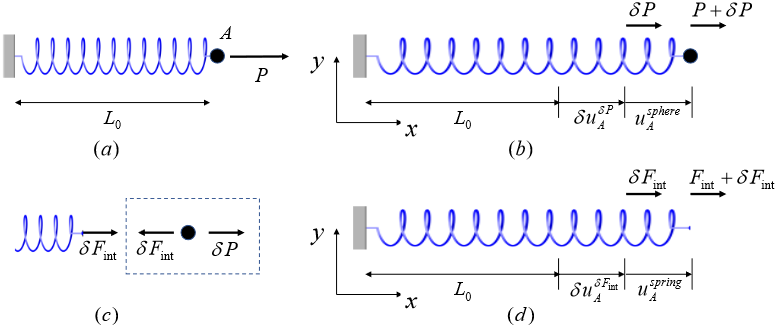
\includegraphics[width=0.666\linewidth]{Figures/Virtual_Force_Springs.png}\par
    $\delta W_e^* = u_A^{sphere} \delta P \rightarrow \delta F_{int}=\delta P$\par 
    $\delta W_e^* = -u_A^{spring} \delta F_{int}$\par 
    $\left(u_A^{sphere}-u_A^{spring}\right)\delta P=0$\par 
    This shows that the sum of the external and internal virtual work due to an 
    external virtual force (or moment) vanishes for structure in static 
    equilibrium, if the displacements and deformations are compatible.

    % ----- Virtual Force ----- %
    \subsection*{Virtual Force Method for Computing Deflections}\par 
    $\delta W_e^*=u \delta P$ or $\delta W_E^* = \theta \delta M$ \par 
    Where $u$ is the real displacement of the point at which the virtual force
    is applied. \par 
    The internal virtual work can be written for a multi-component member as follows:\par 
    $\delta W_{ie}^*=\sum\limits_{N_m} \delta F_{int} \Delta$\par 
    Replace $\delta P$ with 1, $\bar{1}u=\sum\limits_N \bar{f}_{int}\Delta$

    % ----- Truss Example ----- %
    \subsection*{Truss Example}
    
    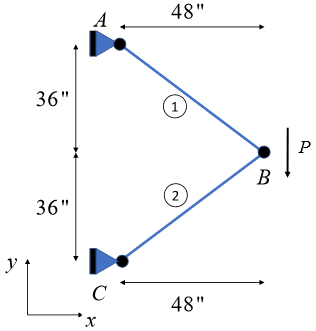
\includegraphics[width=0.5\linewidth]{Figures/Truss_Example_VF.png}

    $\delta W_{ie,bar}^*=\int_L \varepsilon \bar{\sigma} A dx\rightarrow 
    \delta W_{ie,bar}^*=\int_L \frac{\sigma}{E} \bar{\sigma} A dx$\par 
    For the case that the real and virtual stresses are constant in the bar, the 
    above expression can be expressed in terms of the real internal force, $N$, 
    and the virtual force, $\bar{n}$, as follows:\par 
    $\delta W_{ie,bar}^*=\frac{N\bar{n}L}{EA}$\par 
    For a truss composed of multiple bars:\par 
    $\delta W_{ie,truss}^* = \sum\limits_{i=1}^{N_b} \frac{N_i \bar{n}_i L_i}{E_i A_i}$\par 
    Using the balance of external and internal virtual work, i.e. $W_e^*=\delta 
    W_{ie,truss}^*$, and applying a dummy load in a particular direction, the 
    displacement, $d$, at the chosen joint in this direction can be computed by:\par 
    $\bar{1}d=\sum\limits_{i=1}^{N_b} \frac{N_i \bar{n}_i L_i}{E_i A_i}$\par
    Applying to example above:\par 
    \textbf{Step 1:} Compute internal forces, $N_i$, in the bars due to real load $P$. 
    Truss must be statically determinate.\par 
    $N_1=\frac{5}{6}P$ and $N_2=-\frac{5}{6}P$ \par 
    \textbf{Step 2:} Compute internal forces, $\bar{n}_i$, in the bars due to the 
    dummy loads $\bar{1}$. First, we apply a dummy load in the horizontal direction
    to compute the horizontal displacement.\par 
    $\bar{n}_1^u = \frac{5}{8}$ and $\bar{n}_2^u=\frac{5}{8}$ \par 
    Do the same for a vertical dummy load at joint B. \par 
    $\bar{n}_1^v = -\frac{5}{6}$ and $\bar{n}_2^v=\frac{5}{6}$\par 
    \textbf{Step 3:} To evaluate the internal work, summarize in a table: 
     
    \begin{center}
        \begin{tabular}{l|llllll}
            bar & $N_i$ & $\bar{n}_i^u$ & $\bar{n}_i^v$ & $A_i$ & $L_i$ & $E_i$ \\
            \hline
            1 & $\frac{5}{6}P$ & $\frac{5}{8}$ & $-\frac{5}{6}$ & $0.15$ & $60.0$ & $3\cdot 10^6$ \\
            $2$ & $-\frac{5}{6}P$ & $\frac{5}{8}$ & $\frac{5}{6}$ & $0.20$ & $60.0$ & $3\cdot 10^6$ \\
        \end{tabular}
    \end{center}

   \textbf{Step 4:} For each dummy load, evaluate the balance of external and 
   internal forces. \par 
   For the displacement in horizontal:\par 
   $\bar{1}u = \sum\limits_{i=1}^2 \frac{N_i\bar{n}_i^uL_i}{E_iA_i} = 8.33 \cdot 10^{-3} in$ \par 
   Vertical: \par 
   $\bar{1}v = \sum\limits_{i=1}^2 \frac{N_i\bar{n}_i^vL_i}{E_iA_i} = -44.4 \cdot 10^{-3} in$ \par

    % ----- Thermal Loading ----- %
    \subsection*{Thermal Loading}
    Assuming that the material properties are constant in the bar and expressing
    the virtual stress in terms of the internal force, $\bar{n}$, we obtain:\par
    $\delta W_{ie,bar}^{*,thermal}=\alpha \Delta T \bar{n} L$\par 
    Defining an internal force due to differential heating/cooling as:\par
    $N^{thermal} = EA\alpha \Delta T$\par 
    we can write the internal virtual work by replacing the internal force due to
    mechanical loading, $N$, with one for thermal loading, $N^{thermal}$.\par 
    $\delta W_{ie,bar}^* = \frac{N^{thermal}\bar{n}L}{EA}$\par 
    From here follow same procedure as previous.

    % ----- Beam Example ----- %
    \subsection*{Beam Example}\par 
    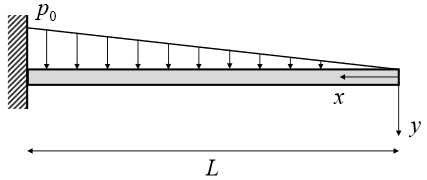
\includegraphics[width=0.5\linewidth]{Figures/Beam_Eample_VF.png}\par 
    First compute internal virtual work of the beam by virtual stress due to a unit dummy load.\par 
    $\delta W_{ie,beam}^*=\int \int \int_V \varepsilon\bar{\sigma}dxdydz$\par 
    Use Hook's Law: $\delta W_{ie,beam}^*=\int \int \int_V \frac{\sigma}{E}\bar{\sigma}dxdydz$\par 
    Recall: $\sigma = -\frac{M}{I}y$\par 
    Finally:\par 
    $\delta W_{ie,beam}^* = \int_L \frac{M\bar{m}}{EI}dx$ where $\bar{m}$ is
    virtual bending moment due to unit dummy load.

    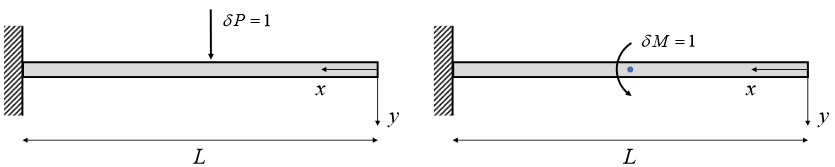
\includegraphics[width=\linewidth]{Figures/Beam_Eample_VF_2.png}\par 
    \textbf{Step 1:} Compute the bending moment due to the real force.\par 
    $M = \frac{p_0 x^3}{6L}$\par 
    \textbf{Step 2:} Compute bending moments due to unit dummy foce and unit
    dummy moment.\par 
    $\bar{m}^v=0$ for $0 \le x < \frac{L}{2}$ and $\bar{m}^v = x - \frac{L}{2}$
    for $\frac{L}{2} \le x \le L$\par 
    $\bar{m}^\phi = 0$ for $0 \le x < \frac{L}{2}$ and $\bar{m}^\phi = -1$
    for $\frac{L}{2} \le x \le L$\par
    \textbf{Step 3:} To compute the displacement and the rotation in the middle
    of the beam, compute the internal work due to the two dummy load cases.\par 
    $v\left(x=\frac{L}{2}\right) = \int_L \frac{M\bar{m}^v}{EI}dx=\int_{l/2}^L \frac{(x-\frac{L}{2})p_0x^3}{6EIL}dx$\par 
    $v\left(\frac{L}{2}\right) = \frac{49p_0L^4}{3840EI}$\par 
    Then do the same thing for $\phi$

    % ----- Direct Stiffness Method ----- %
    \section*{The Direct Stiffness Method}\par 
    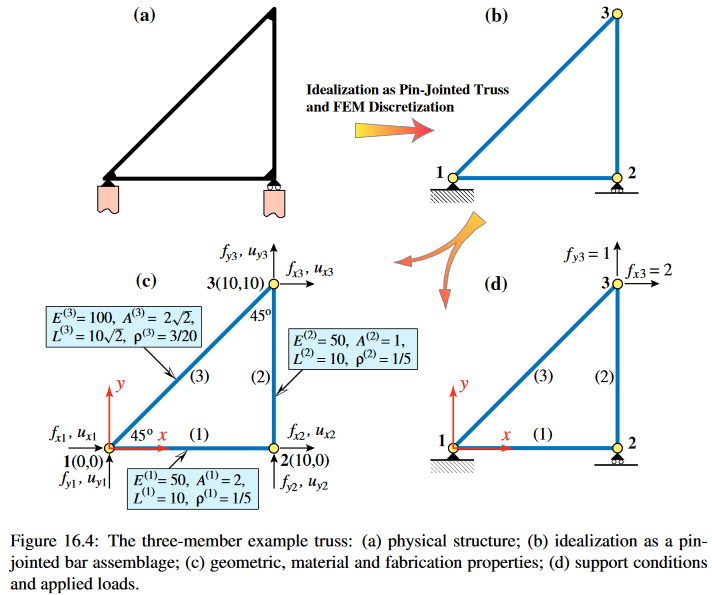
\includegraphics[width=\linewidth]{Figures/DSM1_Example.png}

    \begin{equation*}
        \textbf{f} = 
        \begin{bmatrix}
            f_{x1}\\
            f_{y1}\\
            f_{x2}\\
            f_{y2}\\
            f_{x3}\\
            f_{y3}
        \end{bmatrix}
        \quad
        \textbf{u} = 
        \begin{bmatrix}
            u_{x1}\\
            u_{y1}\\
            u_{x2}\\
            u_{y2}\\
            u_{x3}\\
            u_{y3}
        \end{bmatrix}
    \end{equation*}

    \textbf{Master Stiffness Equations}\par 
    The master stiffness equations relate the joint forces \textbf{f} of the
    complete structure to the joint displacements \textbf{u} of the complete
    structure before specification of support conditions.

    \begin{equation*} 
        \begin{bmatrix}
            f_{x1}\\
            f_{y1}\\
            f_{x2}\\
            f_{y2}\\
            f_{x3}\\
            f_{y3}
        \end{bmatrix}
        =
        \begin{bmatrix}
            K_{x1x1} & K_{x1y1} & K_{x1x2} & K_{x1y2} & K_{x1x3} & K_{x1y3}\\
            K_{y1x1} & K_{y1y1} & K_{y1x2} & K_{y1y2} & K_{y1x3} & K_{y1y3}\\
            K_{x2x1} & K_{x2y1} & K_{x2x2} & K_{x2y2} & K_{x2x3} & K_{x2y3}\\
            K_{y2x1} & K_{y2y1} & K_{y2x2} & K_{y2y2} & K_{y2x3} & K_{y2y3}\\
            K_{x3x1} & K_{x3y1} & K_{x3x2} & K_{x3y2} & K_{x3x3} & K_{x3y3}\\
            K_{y3x1} & K_{y3y1} & K_{y3x2} & K_{y3y2} & K_{y3x3} & K_{y3y3}
        \end{bmatrix}
        \begin{bmatrix}
            u_{x1}\\
            u_{y1}\\
            u_{x2}\\
            u_{y2}\\
            u_{x3}\\
            u_{y3}
        \end{bmatrix} 
    \end{equation*}

    \begin{center}
        \textbf{f = Ku}
    \end{center}
     
    Where \textbf{K} is the master stiffness matrix or the global stiffness matrix.

    \textbf{Breakdown Stage}\par 
    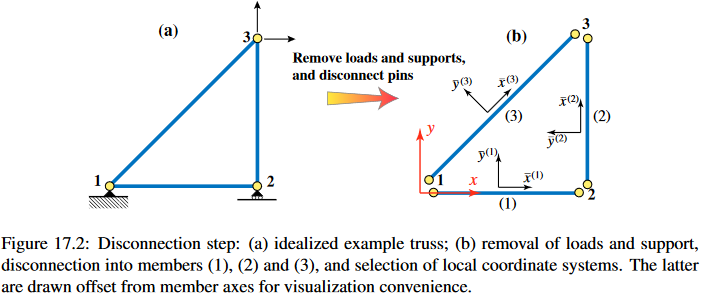
\includegraphics[width=\linewidth]{Figures/breakdown_stage.png}

    Begin by discarding all loads and supports (boundary conditions). Then disconnect
    and disassemble into components. The local coordinate system is $\{ \bar{x},\bar{y}\}$\par 
    \begin{equation*}
        \begin{bmatrix}
            \bar{f}_{xi}\\
            \bar{f}_{yi}\\
            \bar{f}_{xj}\\
            \bar{f}_{yj}
        \end{bmatrix}
        =
        \begin{bmatrix}
            \bar{K}_{xixi} & \bar{K}_{xiyi} & \bar{K}_{xixj} & \bar{K}_{xiyj}\\
            \bar{K}_{yixi} & \bar{K}_{yiyi} & \bar{K}_{yixj} & \bar{K}_{yiyj}\\
            \bar{K}_{xjxi} & \bar{K}_{xjyi} & \bar{K}_{xjxj} & \bar{K}_{xjyj}\\
            \bar{K}_{yjxj} & \bar{K}_{yjyi} & \bar{K}_{yjxj} & \bar{K}_{yjyj}
        \end{bmatrix}
        \begin{bmatrix}
            \bar{u}_{xi}\\
            \bar{u}_{yi}\\
            \bar{u}_{xj}\\
            \bar{u}_{yj}
        \end{bmatrix}
    \end{equation*}

    If membe properties are uniform along its length, $k_s=\frac{EA}{L}$ and,
    consequently, the force-displacement equation is $F=k_sd=\frac{EAd}{l}$ 
    where $F$ is the internal axial force and $d$ is the relative axial displacement,
    which is physically the bar elongation.\par 
    \begin{equation*}
        \bar{\textbf{K}}=\frac{EA}{L}
        \begin{bmatrix}
            1 & 0 & -1 & 0\\
            0 & 0 & 0 & 0 \\
            -1 & 0 & 1 & 0\\
            0 & 0 & 0 & 0
        \end{bmatrix}
    \end{equation*}

    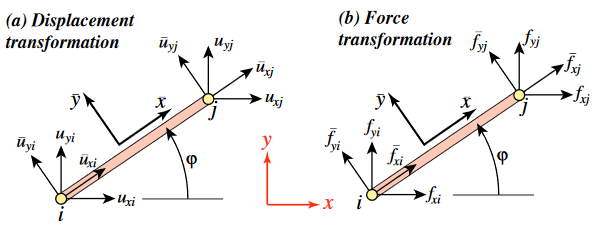
\includegraphics[width=\linewidth]{Figures/DSM1_phi.png}
    
    $c = \cos{\phi}$ and $s = \sin{\phi}$ where $\phi$ is the angle formed by
    $\bar{x}$ and $x$, measured CCW from $x$.\par 
    \begin{equation*}
        \begin{bmatrix}
            \bar{u}_{xi}\\
            \bar{u}_{yi}\\
            \bar{u}_{xj}\\
            \bar{u}_{xy}
        \end{bmatrix}
        =
        \begin{bmatrix}
            c & s & 0 & 0\\
            -s & c & 0 & 0\\
            0 & 0 & c & s\\
            0 & 0 & -s & c
        \end{bmatrix}
        \begin{bmatrix}
            u_{xi}\\
            u_{yi}\\
            u_{xj}\\
            u_{yj}
        \end{bmatrix}
        \quad
        \begin{bmatrix}
            f_{xi}\\
            f_{yi}\\
            f_{xj}\\
            f_{yj}
        \end{bmatrix}
        =
        \begin{bmatrix}
            c & -s & 0 & 0\\
            s & c & 0 & 0\\
            0 & 0 & c & -s\\
            0 & 0 & s & c
        \end{bmatrix}
        \begin{bmatrix}
            \bar{f}_{xi}\\
            \bar{f}_{yi}\\
            \bar{f}_{xj}\\
            \bar{f}_{yj}
        \end{bmatrix}
    \end{equation*}

    \textbf{Global Member Stiffness Equations}\par 
    \begin{equation*}
        \textbf{K}^e = \frac{E^eA^e}{L^e}
        \begin{bmatrix}
            c^2 & sc & -c^2 & -sc\\
            sc & s^2 & -sc & -s^2\\
            -c^2 & -sc & c^2 & sc\\
            -sc & -s^2 & sc & s^2
        \end{bmatrix}
    \end{equation*}

    \textbf{Merging it All}\par 
    \begin{enumerate}
        \item \textit{Compatibility of displacement:} The displacements of all 
                members that meet are a joint are the same.\par
                $u_{x3}^{(2)} = u_{x3}^{(3)}$, $u_{y3}^{(2)} = u_{y3}^{(3)}$
        \item \textit{Force equilibrium:} The sum of internal forces exerted by 
                all members that meet at a joint balances the external force 
                applied to that joint.\par 
                $f_{x3} = f_{x3}^{(2)}+f_{x3}^{(3)}=f_{x3}^{(1)}+f_{x3}^{(2)}+f_{x3}^{(3)}$, 
                $f_{y3} = f_{y3}^{(2)}+f_{y3}^{(3)}=f_{y3}^{(1)}+f_{y3}^{(2)}+f_{y3}^{(3)}$\par
                The addition of $f_{x3}^{(1)}$ does nothing because member 1 is
                not connected to joint 3.
    \end{enumerate}

    Finally, \par 
    $$\textbf{f} = \textbf{f}^{(1)}+\textbf{f}^{(2)}+\textbf{f}^{(3)}=\left(\textbf{K}^{(1)}+\textbf{K}^{(2)}+\textbf{K}^{(3)}\right)\textbf{u} = \textbf{Ku}$$

    \textbf{Solution}

    The best way to account for support conditions is to remove equations that
    are associated with known zero joint displacements from the master system.
    This should result in a system of equations that is solveable for the displacements
    left because the forces at those displacements should be known.

    \textbf{Post Processing}

    Recovering Reaction Forces:\par 
    Multiply complete displacement solution found above by \textbf{K}.\par 
    Recovery of Internal Forces \& stresses:\par 
    The average axial stress $\sigma^e$ is found by dividing $F^e$ by $A^e$.\par 
    The axial force $F^e$ in member $e$ can be found by:\par 
    \begin{equation*}
        d^e=\bar{u}_{xj}^e-\bar{u}_{xi}^e
        \quad
        F^e=\frac{E^eA^e}{L^e}d^e
    \end{equation*}

    % ----- FEM of Beam ----- %
    \subsection*{FEM Analysis of Plane Beam Structure}

    \begin{center}
    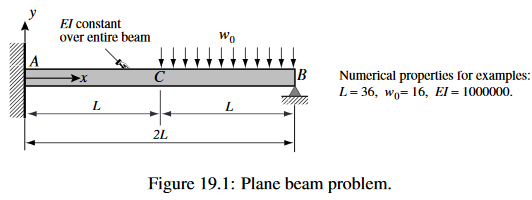
\includegraphics[width=0.75\linewidth]{Figures/FEM_plane_beam.png}\par 
    Beam finite elements are obtained by subdividing beam members longitudinally.
    \begin{equation*}
        \textbf{u}^{(e)} = 
        \begin{bmatrix}
            v_i^{(e)}\\
            \theta_i^{(e)}\\
            v_j^{(e)}\\
            \theta_j^{(e)}
        \end{bmatrix},
        \quad
        \textbf{f}^{(e)} = 
        \begin{bmatrix}
            f_i^{(e)}\\
            m_i^{(e)}\\
            f_j^{(e)}\\
            m_j^{(e)}
        \end{bmatrix}
    \end{equation*}

    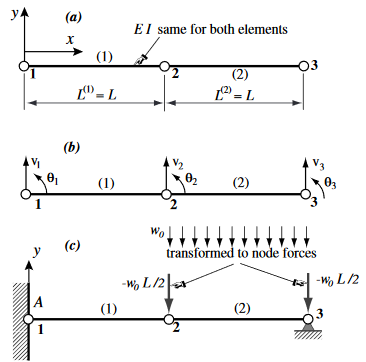
\includegraphics[width=0.5\linewidth]{Figures/FEM_plane_beam_2.png}
    \end{center}

    This beam can be solved like the truss from here on out. See CH 19 page 3 
    for more detailed steps.

    \subsection*{Analytical Solution by Discontinuity Functions}
    \begin{equation*}
        \langle x-a \rangle ^n = \begin{cases} 
            (x-a)^n  & x>a\\
            0 &  x \le a
        \end{cases}
    \end{equation*}

    Begin with:\par 
    $q(x)=-w_0\langle x-L \rangle ^0$\par 
    Then integrate 4 times in x:\par 
    \begin{equation*}
        \begin{array}{llll}
            V(x) & = & -w_0\langle x-L \rangle ^1 + C_1\\
            M(x) & = & -\frac{1}{2}w_0\langle x-L\rangle ^2 + C_1x+C_2\\
            EI\theta (x) = EIv'(x) & = & -\frac{1}{6}w_0\langle x-L\rangle^3+\frac{1}{2}C_1x^2+C_2x+C_3\\
            EIv(x) & = & -\frac{1}{24}w_0\langle x-L\rangle^4 + \frac{1}{6}C_1x^3+\frac{1}{2}C_2x^2+C_3x+C_4
        \end{array}
    \end{equation*}

    Then apply boundary conditions and solve.

    % ----- Single-DOF Oscillator ----- %
    \section*{Free Single-DOF Oscillator}
    A weight of mass $m > 0$ hangs from an extensional spring of stiffness $k /ge 0$
    under gravity acceleration $g$ directed along the spring direction. The weight
    force is $W = mg$. Assume small displacements.

    $$\delta_s=W/k=mg/k$$

    The only degree of freedom is $u = u(t)$.

    \subsection*{Undamped Oscillator}
    Remove the spring and replace it by force $F_s = k(\delta_s+u(t))$. The other
    two forces acting on the mass are its weight and the inertia force $m\ddot{u}(t)$,
    which acts in the opposite direction to the acceleration $\ddot{u}=\ddot{u}(t)$.

    Equilibrium of forces in the $x$ direction requires $m\ddot{u}=W-k(\delta_s+u)=mg-k\delta_s-ku$.
    On cancelling $mg-k\delta_s=0$, we get:

    $$\boxed{m \ddot{u}+ku=0}$$

    This results in the formal form:\par 
    $$\boxed{\ddot{u}+\omega_n^2u=0, \text{ in which } \omega_n=\sqrt\frac{k}{m}}$$
    
    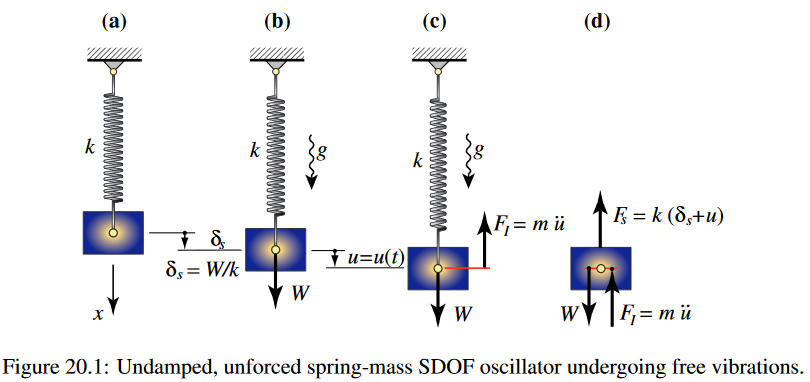
\includegraphics[width=\linewidth]{Figures/SDOF_Undamped.png}

    Solving for $u(t)$:

    \begin{equation*}
        \begin{array}{lll}
            u(t) & = & C_1e^{i\omega_nt}+C_2e^{-i\omega_nt}\\
            u(t) & = & A_1\cos{\omega_nt}+A_2\sin{\omega_nt}\\
            u(t) & = & u_0\cos{\omega_nt}+\frac{v_0}{\omega_n}\sin{\omega_nt}\\
            u(t) & = & U\cos{\omega_nt-\alpha}\\
            U & = & \sqrt{u_0^2 + \left(\frac{v_o}{\omega_n}\right)^2}\\
            \tan{\alpha} & = & \frac{v_0}{\omega_nu_0}
            
        \end{array}
    \end{equation*}

    If the mass is released from rest, and this $v_0 = 0$,\par 
    \begin{center}
        $f_n=\frac{\omega_n}{2\pi}$ and $T_n=\frac{1}{f_n}=\frac{2\pi}{\omega_n}$
    \end{center}
    
    Energy Conservation Property:\par 
    $$T=T_0+\frac{1}{2}m\dot{u}^2 \text{ and } V=V_0+\frac{1}{2}ku^2$$
    $$H=T+V=T_0+U_0=\frac{1}{2}mv_o^2+\frac{1}{2}ku_0^2$$

    \newpage
    \subsection*{Free Vibrations of Viscous-Damped SDOF Oscillator}
    $$\boxed{m\ddot{u}+c\dot{u}+ku=0}$$
    $$w_n=\sqrt{\frac{k}{m}} \text{ , } c=2\xi\omega_nm$$
    $$\boxed{\ddot{u}+2\xi\omega_n\dot{u}+\omega_n^2u=0}$$

    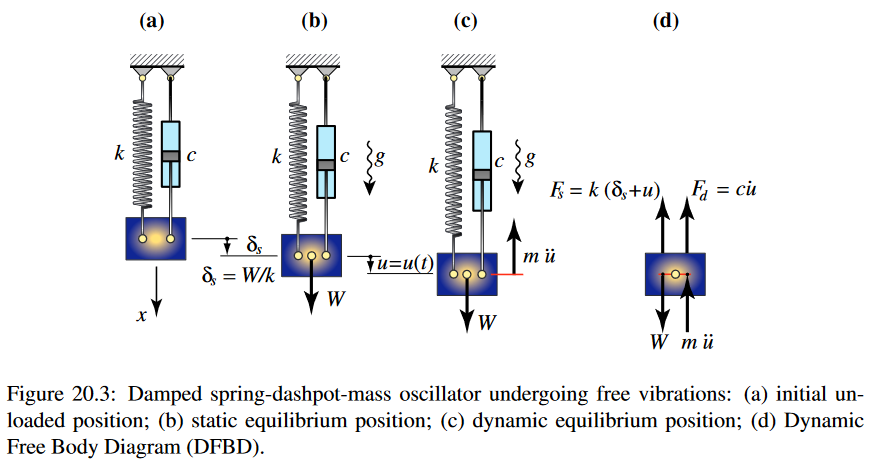
\includegraphics[width=\linewidth]{Figures/SDOF_Ddamped.png}

    Solving for $u(t)$:
    \begin{equation*}
        \begin{array}{lll}
            u(t) & = & Ae^{\lambda t}\\
            0 & = & \lambda^2+2\xi\omega_n\lambda+\omega_n^2\\
            \lambda_{1,2} & = & -\xi\omega_n\pm\omega_n\sqrt{\zeta^2-1}
        \end{array}
    \end{equation*}

    $\xi<1$ \textit{Underdamped case:} Damping is subcritical. The roots $\lambda_{1,2}$
    are complex conjugate. The motion is oscillatory with decreasing amplitude.
    This is the most common case in typical structures.\par 
    $\xi>1$ \textit{Overdampled case:} Damping is called overcritical. The roots
    $\lambda_{1,2}$ are negative real and distinct. The motion is non-oscillatory.
    Its amplitude decays monotonically except possibly for one zero crossing.\par 
    $\xi=1$ \textit{Critically Damped case:} The roots $\lambda_{1,2}$ are negative
    real and coalesce. The motion is non-oscillatory. Its amplitude decays monotonically
    except possibly for one zero crossing. Most rapid decay.

    \textbf{Underdamped Case: $\xi<1$}\par 
    \begin{equation*}
        \begin{array}{lll}
            \lambda_{1,2} & = & -\xi\omega_n\pm i\omega_d\\
            \omega_d & = & \omega_n\sqrt{1-\xi^2}\\
            T_d & = & \frac{2\pi}{\omega_d}\\
            u(t)&=&e^{-\xi\omega_nt}\left(u_0\cos{\omega_dt+\frac{v_0+\xi\omega_nu_0}{\omega_d}\sin{\omega_dt}}\right)
        \end{array}
    \end{equation*}

    \textbf{Critically Damped: $\xi=1$}\par 
    \begin{equation*}
        \begin{array}{lll}
            u(t) & = & [u_0+(v_0+\omega_nu_0)t]e^{-\omega_nt}
        \end{array}
    \end{equation*}

    \textbf{Overdamped Case: $\xi>1$}\par 
    \begin{equation*}
        \begin{array}{lll}
            \omega^* & = & \omega_n\sqrt{\xi^2-1}\\
            u(t) & = & e^{-\xi\omega_nt}\left[u_0\cosh{\omega_*t}+\frac{v_0+\xi\omega_nu_0}{\omega^*}\sinh{\omega^*t}\right]
        \end{array}
    \end{equation*}

    Energy Dissipation: Page 10 of Ch 20.

    \section*{Harmonically Forced SDOF Oscillator}
    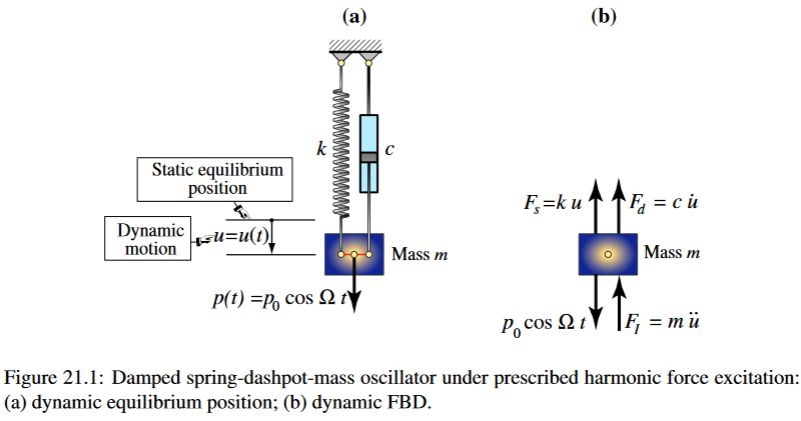
\includegraphics[width=\linewidth]{Figures/forced_oscillator.png}\par 
    Harmonic Excitation Force: $p(t)=p_0\cos{\Omega t}$ where $\Omega$ is the excitation frequency. $u=u(t)$ is the dynamic motion measured
    from the static equilibrium position.
    $$\boxed{m\ddot{u}+c\dot{u}+ku=p_0\cos{\Omega t}}$$
    The complete response will be the sum of the transient (homogeneous) and steady-state (particular) components. If 
    damping is present, after a while the transient part becomes unimportant. 
    $$\boxed{u+p(t)=U\cos{(\Omega t-\alpha)}}$$
    $$\dot{u}_p(t)=-\Omega U \sin{(\Omega t- \alpha)} \text{, } \ddot{u}_p(t) = -\Omega^2U\cos{(\Omega t-\alpha)}$$

    \begin{equation*}
        \begin{array}{l}
            (kU-m\Omega^2U)^2+(c\Omega U)^2 = p_0^2 \text{, } \tan{\alpha}=\frac{c\Omega}{k-m\Omega^2}\\
            U_0=\frac{p_0}{k} \text{, } r = \frac{\Omega}{\omega_n}\\
        \end{array}
    \end{equation*}

    $U_0$ is the displacement that the mass would undergo if a force of mangitude $p_0$ where to be applied statically.
    $$\boxed{D_s(r) = \frac{U(r)}{U_0}=\frac{1}{\sqrt{(1-r^2)^2+(2\xi r)^2}} \text{, } \tan{\alpha(r)}=\frac{2\xi r}{1-r^2}}$$
    $D_s$ is the steady-state magnification factor, also known as gain. The peaks below observed as $r$ is near unity and $\xi << 1$ identify resonance.
    
    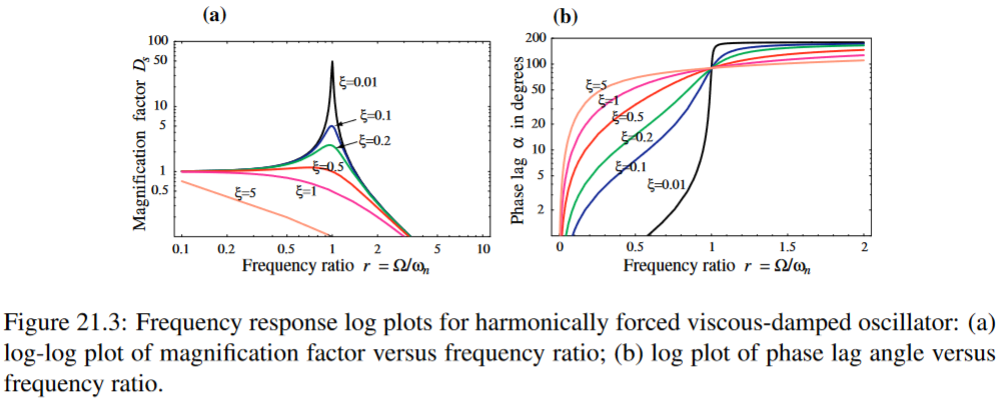
\includegraphics[width=\linewidth]{Figures/freq_response_harmonic_osc.png}

    \textbf{Total Response}
    $$\boxed{u(t)=U_0D_s\cos{\Omega t-\alpha}+u_h(t) \text{, in which } u_h(t) = e^{-\xi \omega_n t}\left(A_1\cos{\omega_nt}+A_2\sin{\omega_nt}\right)}$$

    \subsection*{Response to Harmonic Base Excitation}
    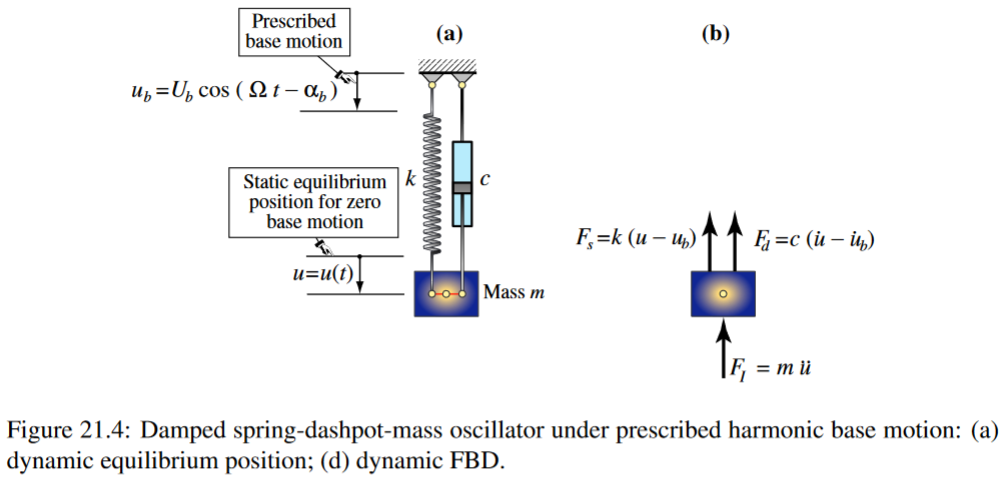
\includegraphics[width=\linewidth]{Figures/harmonic_base.png}\par 
    The base displaces by a prescribed harmonic motion specified as:
    $$u_b(t) = U_b\cos{\Omega t-\alpha}$$
    $$m\ddot{u}+k(u-u_b)+c(\dot{u}-\dot{u}_b)=0$$
    $$\boxed{m\ddot{u}+c\dot{u}+ku=ku_b+c\dot{u}_b}$$
    If the base excitation is harmonic:
    $$\boxed{m\ddot{u}+c\dot{u}+ku=U_b\left[k\cos{(\Omega t-\alpha_b)}+c\Omega\sin{(\Omega t-\alpha_b)}\right]}$$
    If the damping vanishes, $c=0$.

    \section*{MDOF Dynamical Systems}
    


\end{multicols*}  
\end{document}